\documentclass[aspectratio=169]{beamer}

% Theme and Color Setup
\usetheme{Madrid}
\usecolortheme{whale}
\useinnertheme{rectangles}
\useoutertheme{miniframes}

% Additional Packages
\usepackage[utf8]{inputenc}
\usepackage[T1]{fontenc}
\usepackage{graphicx}
\usepackage{booktabs}
\usepackage{listings}
\usepackage{amsmath}
\usepackage{amssymb}
\usepackage{xcolor}
\usepackage{tikz}
\usepackage{pgfplots}
\pgfplotsset{compat=1.18}
\usetikzlibrary{positioning}
\usepackage{hyperref}

% Custom Colors
\definecolor{myblue}{RGB}{31, 73, 125}
\definecolor{mygray}{RGB}{100, 100, 100}
\definecolor{mygreen}{RGB}{0, 128, 0}
\definecolor{myorange}{RGB}{230, 126, 34}
\definecolor{mycodebackground}{RGB}{245, 245, 245}

% Set Theme Colors
\setbeamercolor{structure}{fg=myblue}
\setbeamercolor{frametitle}{fg=white, bg=myblue}
\setbeamercolor{title}{fg=myblue}
\setbeamercolor{section in toc}{fg=myblue}
\setbeamercolor{item projected}{fg=white, bg=myblue}
\setbeamercolor{block title}{bg=myblue!20, fg=myblue}
\setbeamercolor{block body}{bg=myblue!10}
\setbeamercolor{alerted text}{fg=myorange}

% Set Fonts
\setbeamerfont{title}{size=\Large, series=\bfseries}
\setbeamerfont{frametitle}{size=\large, series=\bfseries}
\setbeamerfont{caption}{size=\small}
\setbeamerfont{footnote}{size=\tiny}

% Code Listing Style
\lstdefinestyle{customcode}{
  backgroundcolor=\color{mycodebackground},
  basicstyle=\footnotesize\ttfamily,
  breakatwhitespace=false,
  breaklines=true,
  commentstyle=\color{mygreen}\itshape,
  keywordstyle=\color{blue}\bfseries,
  stringstyle=\color{myorange},
  numbers=left,
  numbersep=8pt,
  numberstyle=\tiny\color{mygray},
  frame=single,
  framesep=5pt,
  rulecolor=\color{mygray},
  showspaces=false,
  showstringspaces=false,
  showtabs=false,
  tabsize=2,
  captionpos=b
}
\lstset{style=customcode}

% Custom Commands
\newcommand{\hilight}[1]{\colorbox{myorange!30}{#1}}
\newcommand{\source}[1]{\vspace{0.2cm}\hfill{\tiny\textcolor{mygray}{Source: #1}}}
\newcommand{\concept}[1]{\textcolor{myblue}{\textbf{#1}}}
\newcommand{\separator}{\begin{center}\rule{0.5\linewidth}{0.5pt}\end{center}}

% Footer and Navigation Setup
\setbeamertemplate{footline}{
  \leavevmode%
  \hbox{%
  \begin{beamercolorbox}[wd=.3\paperwidth,ht=2.25ex,dp=1ex,center]{author in head/foot}%
    \usebeamerfont{author in head/foot}\insertshortauthor
  \end{beamercolorbox}%
  \begin{beamercolorbox}[wd=.5\paperwidth,ht=2.25ex,dp=1ex,center]{title in head/foot}%
    \usebeamerfont{title in head/foot}\insertshorttitle
  \end{beamercolorbox}%
  \begin{beamercolorbox}[wd=.2\paperwidth,ht=2.25ex,dp=1ex,center]{date in head/foot}%
    \usebeamerfont{date in head/foot}
    \insertframenumber{} / \inserttotalframenumber
  \end{beamercolorbox}}%
  \vskip0pt%
}

% Turn off navigation symbols
\setbeamertemplate{navigation symbols}{}

% Title Page Information
\title[Game Playing]{Week 7: Game Playing}
\author[J. Smith]{John Smith, Ph.D.}
\institute[University Name]{
  Department of Computer Science\\
  University Name\\
  \vspace{0.3cm}
  Email: email@university.edu\\
  Website: www.university.edu
}
\date{\today}

% Document Start
\begin{document}

\frame{\titlepage}

\begin{frame}[fragile]
    \titlepage
\end{frame}

\begin{frame}[fragile]
    \frametitle{Overview of Game Playing in AI}
    \begin{block}{Game Playing in AI}
        Game playing is a cornerstone of research in Artificial Intelligence (AI), combining elements of strategy, decision-making, and competition.  
        AI systems that engage in game playing simulate human-like intelligence to outmaneuver opponents. 
        This exploration enhances our understanding of strategic interactions and informs a broad range of applications, from economics to robotics.
    \end{block}
\end{frame}

\begin{frame}[fragile]
    \frametitle{Key Concepts}
    \begin{enumerate}
        \item \textbf{Competitive Scenarios:} 
        Multiple agents make decisions that affect not only their success but also their opponents' outcomes. Examples include chess, poker, and Go.
        
        \item \textbf{Strategic Decision-Making:} 
        Players consider:
        \begin{itemize}
            \item Possible actions and consequences
            \item Predicted reactions of opponents
            \item Optimal strategies to maximize winning chances
        \end{itemize}
        
        \item \textbf{Types of Games:}
        \begin{itemize}
            \item \textbf{Zero-Sum Games:} One player's gain equals another's loss (e.g., chess).
            \item \textbf{Non-Zero-Sum Games:} Scenarios where both can benefit or suffer (e.g., cooperative negotiation scenarios).
        \end{itemize}
    \end{enumerate}
\end{frame}

\begin{frame}[fragile]
    \frametitle{Importance of Strategic Decision-Making}
    \begin{block}{Optimal Strategies}
        AI systems utilize algorithms like Minimax to decide the best move:
        \begin{lstlisting}[language=Python]
def minimax(depth, is_maximizing_player):
    if depth == 0 or game_is_over():
        return evaluate_board()
    
    if is_maximizing_player:
        max_eval = float('-inf')
        for each child in get_children():
            eval = minimax(depth - 1, False)
            max_eval = max(max_eval, eval)
        return max_eval
    else:
        min_eval = float('inf')
        for each child in get_children():
            eval = minimax(depth - 1, True)
            min_eval = min(min_eval, eval)
        return min_eval
        \end{lstlisting}
    \end{block}

    \begin{block}{Real-World Applications}
        These strategies extend to economics, resource management, and multi-agent systems requiring decision-making under uncertainty.
    \end{block}
\end{frame}

\begin{frame}[fragile]
    \frametitle{Conclusion}
    \begin{itemize}
        \item Game playing in AI models complex decision-making processes.
        \item Strategic decisions impact outcomes and reveal insights on competitor behavior.
        \item Algorithms like Minimax and Alpha-Beta Pruning are essential for crafting winning strategies.
    \end{itemize}
    
    Understanding game playing within AI provides insights into tactics, foresight, and adaptability in both human players and algorithms.
\end{frame}

\begin{frame}[fragile]
    \frametitle{Game Playing Strategies - Overview}
    In the realm of Artificial Intelligence (AI), game playing strategies are essential for decision-making processes, especially when competing against an opponent. 
    \begin{itemize}
        \item Strategies maximize a player's chances of winning while anticipating the opponent's moves.
        \item Focus on competitive scenarios where player choices significantly impact outcomes.
    \end{itemize}
\end{frame}

\begin{frame}[fragile]
    \frametitle{Game Playing Strategies - Key Concepts}
    \begin{enumerate}
        \item \textbf{Zero-Sum Games:}
        \begin{itemize}
            \item \textbf{Definition:} A situation where one player's gain is balanced by another's loss; the total utility is constant.
            \item \textbf{Example:} Chess – if Player A wins (+1), Player B loses (-1); thus, the total outcome is zero.
        \end{itemize}
        
        \item \textbf{Optimal Strategies:}
        \begin{itemize}
            \item \textbf{Definition:} The best decision-making strategy that maximizes outcomes, considering the opponent's optimal play.
            \item \textbf{Importance:} Essential for determining victory in competitive environments; players must evaluate possible moves effectively.
        \end{itemize}
    \end{enumerate}
\end{frame}

\begin{frame}[fragile]
    \frametitle{Game Playing Strategies - Illustrations and Conclusion}
    \begin{itemize}
        \item \textbf{Game Trees:}
        \begin{itemize}
            \item Graphical representation of possible moves; nodes represent game states, and edges show possible moves.
            \item Example: In tic-tac-toe, nodes depict board configurations, illustrating strategic alternatives.
        \end{itemize}

        \item \textbf{Example of Strategy Evaluation:}
        \begin{itemize}
            \item In a game where players pick numbers from 1 to 10, players should always choose the highest available number to optimize their score.
        \end{itemize}
    \end{itemize}
    
    \textbf{Conclusion:} 
    Understanding game strategies in AI, especially zero-sum games and optimal strategies, is crucial for developing smart agents in competitive environments. Mastering these concepts lays the foundation for implementing effective decision-making algorithms.
\end{frame}

\begin{frame}[fragile]
    \frametitle{The Minimax Algorithm}
    The Minimax algorithm is a decision-making and game theory strategy used in two-player, zero-sum games. The purpose of this algorithm is to minimize possible losses while maximizing potential gains.
\end{frame}

\begin{frame}[fragile]
    \frametitle{Key Concepts of Minimax}
    \begin{itemize}
        \item \textbf{Optimal Strategy:} Ensures players make the best possible moves.
        \item \textbf{Game Tree:} Represents game states and possible moves.
        \item \textbf{Min and Max Levels:}
        \begin{itemize}
            \item \textbf{Max Player:} Aims for the highest score.
            \item \textbf{Min Player:} Aims to minimize the score of the Max player.
        \end{itemize}
    \end{itemize}
\end{frame}

\begin{frame}[fragile]
    \frametitle{How Minimax Works}
    \begin{enumerate}
        \item \textbf{Tree Construction:} Start from the current state and generate all possible moves.
        \item \textbf{Evaluation of Leaf Nodes:} Assign values to terminal nodes:
            \begin{itemize}
                \item Win = +1
                \item Loss = -1
                \item Draw = 0
            \end{itemize}
        \item \textbf{Backward Evaluation:} Recursively evaluate and propagate values up the tree.
        \item \textbf{Choosing the Optimal Move:} The root node's value indicates the best move.
    \end{enumerate}
\end{frame}

\begin{frame}[fragile]
    \frametitle{Example: Tic-Tac-Toe}
    \textbf{Current Board State:}
    \begin{verbatim}
     X | O |  
    -----------
     X | O |  
    -----------
       |   | X
    \end{verbatim}
    \begin{itemize}
        \item Max player (X) evaluates potential moves and constructs a game tree.
        \item Leaves are evaluated based on potential outcomes:
            \begin{itemize}
                \item +1 (X wins)
                \item 0 (Draw)
                \item -1 (O wins)
            \end{itemize}
    \end{itemize}
\end{frame}

\begin{frame}[fragile]
    \frametitle{Conclusion and Key Points}
    \begin{itemize}
        \item Minimax is effective for deterministic games with perfect information.
        \item \textbf{Alpha-Beta Pruning:} Enhances Minimax by eliminating non-critical branches for faster evaluations.
    \end{itemize}
    In summary, the Minimax algorithm is foundational for AI decision-making in competitive games, providing a framework for successful strategies.
\end{frame}

\begin{frame}
    \frametitle{Minimax Algorithm Mechanics}
    \begin{block}{Learning Objectives}
        \begin{itemize}
            \item Understand how the Minimax algorithm evaluates possible moves in two-player games.
            \item Familiarize yourself with the tree structure representing game states.
            \item Learn how the algorithm traverses this tree to make optimal decisions.
        \end{itemize}
    \end{block}
\end{frame}

\begin{frame}
    \frametitle{The Minimax Algorithm Explained}
    \begin{block}{Definition}
        The \textbf{Minimax algorithm} is a decision-making tool used in two-player games, designed to minimize the possible loss in a worst-case scenario. 
    \end{block}
    \begin{block}{Key Mechanism}
        By analyzing potential moves, the algorithm maximizes a player's chances of winning.
    \end{block}
\end{frame}

\begin{frame}
    \frametitle{Tree Structure of Game States}
    \begin{itemize}
        \item \textbf{Game Tree Representation}: 
        \begin{itemize}
            \item \textbf{Nodes}: Represent game states (positions of pieces).
            \item \textbf{Edges}: Represent possible moves transitioning between states.
        \end{itemize}
    \end{itemize}
    \begin{block}{Example}
        In Tic-Tac-Toe, each turn creates new branches depicting different arrangements of Xs and Os.
    \end{block}
\end{frame}

\begin{frame}
    \frametitle{Traversing the Game Tree}
    \begin{enumerate}
        \item \textbf{Node Evaluation}:
            \begin{itemize}
                \item Leaf node outcomes: Win $\rightarrow$ +1, Loss $\rightarrow$ -1, Draw $\rightarrow$ 0.
                \item Evaluation reflects the desirability of a game state.
            \end{itemize}
        \item \textbf{Backpropagation of Values}:
            \begin{itemize}
                \item Maximizing player's turn: Set node value to the maximum of child nodes.
                \item Minimizing player's turn: Set node value to the minimum of child nodes.
            \end{itemize}
            \begin{block}{Example}
                If X has a potential outcome of +1 and O can only return -1, X chooses +1.
            \end{block}
    \end{enumerate}
\end{frame}

\begin{frame}[fragile]
    \frametitle{Optimal Move Selection}
    \begin{itemize}
        \item Continue evaluations until reaching the root of the tree.
        \item Maximizing player chooses the move leading to the best outcome.
    \end{itemize}
\end{frame}

\begin{frame}
    \frametitle{Key Points to Emphasize}
    \begin{itemize}
        \item \textbf{Depth-first Search}: Minimax uses a depth-first strategy to explore branches thoroughly.
        \item \textbf{Optimal Play Assumption}: Both players play optimally to maximize their scores while minimizing their opponent's.
        \item \textbf{Complexity}: Can be computationally expensive; heuristics and pruning techniques like \textbf{Alpha-Beta Pruning} can help.
    \end{itemize}
\end{frame}

\begin{frame}[fragile]
    \frametitle{Pseudocode for Minimax Algorithm}
    \begin{lstlisting}[language=Python]
def minimax(node, depth, isMaximizing):
    if depth == 0 or terminal_node(node):
        return evaluate(node)  # Return heuristic value of node

    if isMaximizing:
        maxEval = float('-inf')
        for child in get_children(node):
            eval = minimax(child, depth - 1, False)
            maxEval = max(maxEval, eval)
        return maxEval
    else:
        minEval = float('inf')
        for child in get_children(node):
            eval = minimax(child, depth - 1, True)
            minEval = min(minEval, eval)
        return minEval
    \end{lstlisting}
\end{frame}

\begin{frame}
    \frametitle{Conclusion}
    The Minimax algorithm is a powerful tool to ensure optimal decisions in two-player games, relying on game tree structures and strategic evaluations of future possibilities. By mastering these mechanics, players can significantly enhance their gameplay strategy.
\end{frame}

\begin{frame}[fragile]
    \frametitle{Minimax Example - Learning Objectives}
    \begin{itemize}
        \item Understand the implementation of the Minimax algorithm through a simple game scenario.
        \item Learn how to evaluate game states based on potential outcomes.
    \end{itemize}
\end{frame}

\begin{frame}[fragile]
    \frametitle{Minimax Example - Introduction to Minimax}
    \begin{block}{Introduction}
        The Minimax algorithm is a decision-making strategy used in zero-sum games, such as Tic-Tac-Toe, where one player's gain is another player's loss. The objective of Minimax is to minimize the possible loss in a worst-case scenario.
    \end{block}
\end{frame}

\begin{frame}[fragile]
    \frametitle{Minimax Example - Worked Example: Tic-Tac-Toe}
    \textbf{Game Setup}:
    \begin{itemize}
        \item \textbf{Players}: Player 1 (X) and Player 2 (O)
        \item \textbf{Objective}: Get three of your marks in a row (horizontally, vertically, or diagonally).
        \item \textbf{Initial Board State}:
    \end{itemize}
    \begin{center}
        \begin{tabular}{|c|c|c|}
            \hline
            & & \\ \hline
            & & \\ \hline
            & & \\ \hline
        \end{tabular}
    \end{center}
\end{frame}

\begin{frame}[fragile]
    \frametitle{Minimax Example - Game Tree Exploration}
    \begin{block}{Player 1's Turn: Initial Board State}
        \begin{center}
            \begin{tabular}{|c|c|c|}
                \hline
                X & O & \\ \hline
                & X & \\ \hline
                & O & \\ \hline
            \end{tabular}
        \end{center}
    \end{block}
    
    \textbf{Possible Moves for Player 1 (X)}:
    \begin{enumerate}
        \item Place X in Row 3, Column 1.
        \item Place X in Row 2, Column 3.
    \end{enumerate}
\end{frame}

\begin{frame}[fragile]
    \frametitle{Minimax Example - Scoring the Outcomes}
    \begin{block}{If Player 1 places X in Row 3, Column 1}
        \begin{center}
            \begin{tabular}{|c|c|c|}
                \hline
                X & O & \\ \hline
                O & X & \\ \hline
                X & O & \\ \hline
            \end{tabular}
        \end{center}
        \textbf{Score}: Draw (Score = 0)
    \end{block}
    
    \begin{block}{If Player 1 places X in Row 2, Column 3}
        \begin{center}
            \begin{tabular}{|c|c|c|}
                \hline
                X & O & \\ \hline
                & X & X \\ \hline
                O & O & \\ \hline
            \end{tabular}
        \end{center}
        \textbf{Score}: No immediate winning move but possibilities exist (Score > 0).
    \end{block}
\end{frame}

\begin{frame}[fragile]
    \frametitle{Minimax Example - Minimax Logic}
    \begin{itemize}
        \item Calculate the Minimax values for each possible move:
        \begin{itemize}
            \item If the opponent can surely win, return -1 (worst-case).
            \item If there's no way to lose (resulting in a draw), score as 0.
            \item Winning scenarios score as 1.
        \end{itemize}
    \end{itemize}
    
    \textbf{Final Decision}: Minimax evaluates all possible game outcomes and selects the move that maximizes Player 1's score while minimizing potential losses.
\end{frame}

\begin{frame}[fragile]
    \frametitle{Minimax Example - Key Points and Conclusion}
    \begin{itemize}
        \item \textbf{Optimal Play}: The Minimax algorithm assumes opponents will play optimally.
        \item \textbf{Game Tree Structure}: Understanding and generating a game tree helps simulate outcomes effectively.
        \item \textbf{Complexity}: Works well for simple games like Tic-Tac-Toe but may diminish with complex branching factors.
    \end{itemize}
    
    \begin{block}{Conclusion}
        The Minimax algorithm empowers strategic play in turn-based games by simulating potential outcomes. Mastering this concept provides foundational skills for advanced algorithms in artificial intelligence.
    \end{block}
\end{frame}

\begin{frame}[fragile]
    \frametitle{Minimax Example - Note to Students}
    \begin{block}{Practice}
        Implement the Minimax algorithm with different scenarios in Tic-Tac-Toe. Create visual representations of game trees to reinforce your understanding.
    \end{block}
\end{frame}

\begin{frame}[fragile]
    \frametitle{Limitations of Minimax - Overview}
    \begin{block}{Overview of Minimax Algorithm}
        The Minimax algorithm is a decision-making algorithm used in game theory and artificial intelligence, particularly in two-player games. It tries to minimize the possible loss for a worst-case (maximum loss) scenario.
    \end{block}
\end{frame}

\begin{frame}[fragile]
    \frametitle{Limitations of Minimax - Key Limitations}
    \begin{enumerate}
        \item \textbf{Computational Complexity}
        \begin{itemize}
            \item \textbf{Exponential Growth:} O(b\textsuperscript{d}), where:
            \begin{itemize}
                \item b = branching factor
                \item d = depth of the game tree
            \end{itemize}
            \item e.g., In chess, b $\approx$ 35, d $\approx$ 80 ($\sim$35\textsuperscript{80} is massive).
        \end{itemize}

        \item \textbf{Inefficiency in Large Game Trees}
        \begin{itemize}
            \item \textbf{Search Space Explosion:} Manageability issues with increasing depth and branching factor.
            \item \textbf{Time Constraints:} Real-time decisions may not be feasible.
        \end{itemize}
    \end{enumerate}
\end{frame}

\begin{frame}[fragile]
    \frametitle{Limitations of Minimax - Additional Limitations}
    \begin{enumerate}[resume]
        \item \textbf{Static Evaluation Function Dependency}
        \begin{itemize}
            \item \textbf{Quality of Evaluation:} The algorithm relies on heuristic evaluations; poor quality impacts performance.
            \item e.g., In chess, underestimating a piece's strategic position can lead to missed opportunities.
        \end{itemize}

        \item \textbf{No Handling of Draws or Stalemates}
        \begin{itemize}
            \item Minimax does not account for potential draws, affecting decision-making.
        \end{itemize}

        \item \textbf{Lack of Adaptivity}
        \begin{itemize}
            \item Strategies are fixed after initial analysis; re-evaluation of the entire tree is needed for adaptation.
        \end{itemize}
    \end{enumerate}
\end{frame}

\begin{frame}[fragile]
    \frametitle{Limitations of Minimax - Example and Conclusion}
    \begin{block}{Illustrative Example}
        For a simple game like Tic-Tac-Toe:
        \begin{itemize}
            \item Depth involves multiple layers of possible moves.
            \item About 5,478 valid game positions; feasible for Tic-Tac-Toe but challenging for larger games like chess.
        \end{itemize}
    \end{block}

    \begin{block}{Conclusion}
        While foundational in AI game playing, Minimax's prohibitive computational complexity and inefficiencies make it less effective for complex games without enhancements.
    \end{block}

    \begin{block}{Key Takeaway}
        Understanding the limitations of the Minimax algorithm highlights the need for improvements, such as Alpha-Beta Pruning.
    \end{block}
\end{frame}

\begin{frame}[fragile]
    \frametitle{Introduction to Alpha-Beta Pruning - Overview}
    \begin{block}{Overview of Alpha-Beta Pruning}
        Alpha-Beta Pruning is an optimization technique used with the Minimax algorithm in decision-making scenarios, particularly in game-playing AI. 
        While Minimax seeks to minimize potential loss for a worst-case scenario, Alpha-Beta Pruning enhances efficiency by eliminating branches in the game tree that do not need to be explored.
    \end{block}
\end{frame}

\begin{frame}[fragile]
    \frametitle{Introduction to Alpha-Beta Pruning - The Need for Optimization}
    \begin{block}{The Need for Optimization}
        \begin{itemize}
            \item The Minimax algorithm can be computationally expensive, especially in games with a large branching factor (e.g., chess).
            \item This results in an exponential growth of possible game states, leading to performance bottlenecks.
            \item Alpha-Beta Pruning addresses these limitations by:
            \begin{itemize}
                \item Reducing the number of nodes evaluated in the game tree.
                \item Allowing the algorithm to explore deeper levels of the tree efficiently.
            \end{itemize}
        \end{itemize}
    \end{block}
\end{frame}

\begin{frame}[fragile]
    \frametitle{Introduction to Alpha-Beta Pruning - Key Concepts and Benefits}
    \begin{block}{Key Concepts}
        \begin{itemize}
            \item \textbf{Alpha (α)}: The best (highest-value) choice found so far at any point along the path to the root for the maximizer.
            \item \textbf{Beta (β)}: The best (lowest-value) choice found so far at any point along the path to the root for the minimizer.
        \end{itemize}
    \end{block}
    
    \begin{block}{Benefits of Alpha-Beta Pruning}
        \begin{itemize}
            \item \textbf{Efficiency}: In the best-case scenario, time complexity can be reduced from $O(b^d)$ to $O(b^{d/2})$, where $b$ is the branching factor and $d$ is the depth of the tree.
            \item \textbf{Deeper Searches}: Fewer nodes evaluated allows the algorithm to examine deeper game states within the same timeframe.
        \end{itemize}
    \end{block}
\end{frame}

\begin{frame}[fragile]
    \frametitle{Introduction to Alpha-Beta Pruning - Methodology and Example}
    \begin{block}{How It Works}
        \begin{itemize}
            \item As Minimax explores the tree, it keeps track of the alpha and beta values.
            \item If a node is found that is worse than previously examined nodes, the branch is pruned away. 
            \item This optimization saves time by not exploring unnecessary paths.
        \end{itemize}
    \end{block}
    
    \begin{block}{Example}
        \begin{verbatim}
                MAX
               /   \
             3     MIN
                   /  \
                  5    6
               /   \
             2     1
        \end{verbatim}
        In this tree, the MAX player knows that the MIN player will choose 5 over 6, thus the node with 6 can be pruned.
    \end{block}
\end{frame}

\begin{frame}[fragile]
    \frametitle{Introduction to Alpha-Beta Pruning - Summary & Next Steps}
    \begin{block}{Summary & Key Points}
        \begin{itemize}
            \item Alpha-Beta Pruning optimizes the Minimax algorithm by removing irrelevant branches.
            \item It permits faster decision-making in complex game environments.
            \item Understanding alpha and beta values is crucial for effective implementation.
        \end{itemize}
    \end{block}
    
    \begin{block}{Next Steps}
        In the following slide, we will delve deeper into the mechanics of the Alpha-Beta Pruning algorithm, exploring its implementation and real-world applications.
    \end{block}
\end{frame}

\begin{frame}[fragile]
    \frametitle{Alpha-Beta Mechanics - Concept Overview}
    \begin{block}{Alpha-Beta Pruning}
        Alpha-beta pruning is an optimization technique for the Minimax algorithm, widely used in adversarial games.
    \end{block}
    \begin{itemize}
        \item Reduces the number of nodes evaluated in the game tree
        \item Minimizes computational resources and time
        \item Arrives at the same optimal outcome
    \end{itemize}
\end{frame}

\begin{frame}[fragile]
    \frametitle{Alpha-Beta Mechanics - How Does It Work?}
    \begin{enumerate}
        \item \textbf{Initialization}:
            \begin{itemize}
                \item \textbf{Alpha ($\alpha$)}: Best score (minimum) for the maximizing player.
                \item \textbf{Beta ($\beta$)}: Best score (maximum) for the minimizing player.
            \end{itemize}
        \item \textbf{Tree Traversal}:
            \begin{itemize}
                \item If node's value $\leq \alpha$: prune branch.
                \item If node's value $\geq \beta$: prune branch.
            \end{itemize}
    \end{enumerate}
\end{frame}

\begin{frame}[fragile]
    \frametitle{Alpha-Beta Mechanics - Example}
    Consider the following game tree:

    \begin{center}
    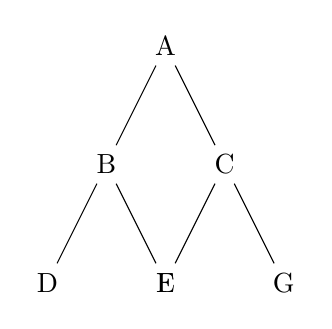
\begin{tikzpicture}
    \node {A}
        child {node {B}
            child {node {D}}
            child {node {E}}}
        child {node {C}
            child {node {F}}
            child {node {G}}};
    \end{tikzpicture}
    \end{center}

    \begin{itemize}
        \item If we find a value for D of 3, and $\alpha = 2$:
            \begin{itemize}
                \item We can prune exploration of node B's right child (E).
            \end{itemize}
    \end{itemize}
\end{frame}

\begin{frame}[fragile]
    \frametitle{Alpha-Beta Mechanics - Benefits}
    \begin{itemize}
        \item \textbf{Efficiency}: Can reduce node evaluations by about 50\% in many cases.
        \item \textbf{Performance}: Handles deeper search trees, improving AI in complex games.
        \item \textbf{Optimal Decisions}: Maintains optimal decision-making like Minimax.
    \end{itemize}
\end{frame}

\begin{frame}[fragile]
    \frametitle{Alpha-Beta Mechanics - Pseudocode}
    \begin{lstlisting}[language=Python]
function AlphaBeta(node, depth, α, β, maximizingPlayer):
    if depth == 0 or node is a terminal node:
        return evaluate(node)
    
    if maximizingPlayer:
        value = -∞
        for each child of node:
            value = max(value, AlphaBeta(child, depth - 1, α, β, false))
            α = max(α, value)
            if β ≤ α:
                break // β cut-off
        return value
    else:
        value = +∞
        for each child of node:
            value = min(value, AlphaBeta(child, depth - 1, α, β, true))
            β = min(β, value)
            if β ≤ α:
                break // α cut-off
        return value
    \end{lstlisting}
\end{frame}

\begin{frame}[fragile]
    \frametitle{Introduction to Alpha-Beta Pruning}
    \begin{block}{Definition}
        Alpha-Beta Pruning is an optimization technique used in the Minimax algorithm for game-playing AI. It selectively prunes branches in the game tree that do not affect the final decision, leading to fewer nodes evaluated.
    \end{block}
\end{frame}

\begin{frame}[fragile]
    \frametitle{Recap of the Minimax Algorithm}
    \begin{itemize}
        \item The Minimax algorithm minimizes the potential loss in a worst-case scenario against an optimally playing opponent.
        \item Each node represents a game state and is assigned scores based on terminal outcomes.
    \end{itemize}
\end{frame}

\begin{frame}[fragile]
    \frametitle{How Alpha-Beta Pruning Works}
    \begin{itemize}
        \item **Alpha (α)**: The minimum score the maximizing player can guarantee.
        \item **Beta (β)**: The maximum score the minimizing player can guarantee.
    \end{itemize}
    \begin{block}{Pruning Conditions}
        \begin{itemize}
            \item If a node's score is worse than the current β value for the minimizing player, that branch can be pruned.
            \item If a node's score is better than the current α value for the maximizing player, the remaining branches can also be pruned.
        \end{itemize}
    \end{block}
\end{frame}

\begin{frame}[fragile]
    \frametitle{Example Game Tree}
    Consider a sample game tree with depth 3:
    \begin{center}
        \includegraphics[width=0.5\textwidth]{game_tree.png}
    \end{center}
    Assuming terminal node values are:
    \begin{itemize}
        \item D = 3, E = 5, F = 6
        \item G = 9, H = 1, I = 4
    \end{itemize}
\end{frame}

\begin{frame}[fragile]
    \frametitle{Standard Minimax Approach}
    \begin{enumerate}
        \item Evaluate node A by selecting values from its child nodes B and C.
        \item B's values:
        \begin{equation}
            \text{Min}(B) = \min(3, 5, 6) = 3
        \end{equation}
        \item C's values:
        \begin{equation}
            \text{Min}(C) = \min(9, 1, 4) = 1
        \end{equation}
        \item Node A selects the maximum:
        \begin{equation}
            \text{Max}(A) = \max(3, 1) = 3
        \end{equation}
    \end{enumerate}
\end{frame}

\begin{frame}[fragile]
    \frametitle{Alpha-Beta Pruning Approach}
    \begin{enumerate}
        \item Initialize α = $-\infty$ and β = $+\infty$ at node A.
        \item Evaluate node B:
        \begin{itemize}
            \item For D: $\alpha = \max(-\infty, 3) \rightarrow \alpha = 3$
            \item For E: $\alpha = \max(3, 5) \rightarrow \alpha = 5$
            \item For F: $\alpha = \max(5, 6) \rightarrow \alpha = 6$ (Result: Min(B) = 6)
        \end{itemize}
        \item Evaluate node C:
        \begin{itemize}
            \item For G: $\beta = \min(+\infty, 9) \rightarrow \beta = 9$
            \item For H: Prune because 1 < 6; do not evaluate I.
        \end{itemize}
        \item Final decision at A:
        \begin{equation}
            \text{Max}(A) = \max(6, 1) = 6
        \end{equation}
    \end{enumerate}
\end{frame}

\begin{frame}[fragile]
    \frametitle{Key Points}
    \begin{itemize}
        \item **Efficiency**: Alpha-Beta Pruning significantly reduces the number of nodes evaluated.
        \item **Optimality**: The algorithm maintains the same accuracy as the standard Minimax, computing the best move efficiently.
    \end{itemize}
\end{frame}

\begin{frame}[fragile]
    \frametitle{Conclusion}
    Alpha-Beta Pruning optimizes the Minimax algorithm by eliminating unnecessary evaluations, enhancing decision-making speed in game-playing AI significantly.
\end{frame}

\begin{frame}[fragile]
    \frametitle{Strategic Considerations in Game Playing - Overview}
    Implementing AI in game scenarios involves multiple strategic considerations, primarily focusing on \textbf{risk assessment} and \textbf{opponent modeling}. These concepts are vital for developing effective game strategies and improving decision-making.
\end{frame}

\begin{frame}[fragile]
    \frametitle{Strategic Considerations in Game Playing - Risk Assessment}
    \begin{block}{Definition}
        Risk assessment involves evaluating the potential losses or gains associated with different moves or strategies in a game.
    \end{block}
    \begin{block}{Importance}
        Helps in choosing the best action by analyzing both short-term gains and long-term consequences.
    \end{block}
    
    \textbf{Example:} In chess, a player may assess the risk of sacrificing a rook to capture a more valuable piece. By using calculations, the player can evaluate the potential advantage of the overall position, weighing the risk against the expected benefits.

    \begin{itemize}
        \item \textbf{Probabilities:} Assess the likelihood of different outcomes based on available moves.
        \item \textbf{Payoff Matrices:} Use matrices to evaluate possible moves and their associated risks versus rewards.
    \end{itemize}
\end{frame}

\begin{frame}[fragile]
    \frametitle{Strategic Considerations in Game Playing - Opponent Modeling}
    \begin{block}{Definition}
        Opponent modeling is the process of creating a representation of an opponent’s strategies, styles, and tendencies to anticipate their moves effectively.
    \end{block}
    \begin{block}{Importance}
        Understanding your opponent’s behavior can guide AI in selecting counter-strategies, making it more competitive.
    \end{block}
    
    \textbf{Example:} In poker, an AI can observe the betting patterns of human players and adjust its strategy based on their tendencies, such as being overly aggressive or conservative.

    \begin{itemize}
        \item \textbf{Modeling Techniques:}
            \begin{itemize}
                \item \textbf{Behavioral Analysis:} Track and analyze previous moves and decisions of the opponent to identify patterns.
                \item \textbf{Machine Learning:} Train models using historical game data to predict the opponent's future actions.
            \end{itemize}
    \end{itemize}
\end{frame}

\begin{frame}[fragile]
    \frametitle{Applications of Game Playing AI - Overview}
    \begin{block}{What is Game-Playing AI?}
        Game-playing AI refers to algorithms and techniques used to simulate human decision-making in strategic games. These applications showcase the potential of AI and serve as benchmarks for broader AI challenges.
    \end{block}
\end{frame}

\begin{frame}[fragile]
    \frametitle{Applications of Game Playing AI - Chess}
    \begin{itemize}
        \item \textbf{Concept}: Deep Blue, created by IBM, was the first AI to defeat a reigning world chess champion, Garry Kasparov, in 1997.
        \item \textbf{Algorithm}: The Minimax algorithm, enhanced with Alpha-Beta pruning, evaluates optimal moves by examining possible game states.
        \item \textbf{Key Point}: Chess AI balances brute force (searching many possible move sequences) with strategic assessment (weighing the value of those moves).
    \end{itemize}
    \begin{block}{Illustration}
        Imagine a tree structure where each node represents a game state. The Minimax algorithm prunes branches that won’t affect the final decision, making it efficient.
    \end{block}
\end{frame}

\begin{frame}[fragile]
    \frametitle{Applications of Game Playing AI - Go and Modern Video Games}
    \begin{block}{Go}
        \begin{itemize}
            \item \textbf{Concept}: Go, an ancient board game, is regarded as more complex than chess due to its vast search space.
            \item \textbf{Algorithm}: AlphaGo, developed by DeepMind, utilizes neural networks and Monte Carlo Tree Search (MCTS) to predict the best move based on extensive data learning.
            \item \textbf{Key Point}: MCTS allows AI to simulate numerous potential game paths without exhaustive computation, facilitating strategic planning and adaptability.
        \end{itemize}
        \begin{block}{Example}
            AlphaGo's success against human champions highlighted the effectiveness of combining deep learning with traditional search techniques.
        \end{block}
    \end{block}

    \begin{block}{Modern Video Games}
        \begin{itemize}
            \item \textbf{Concept}: AI in modern video games manages non-player characters (NPCs) and enhances player experiences.
            \item \textbf{Algorithm}: Different game genres may use pathfinding algorithms (e.g., A* algorithm) or decision trees for NPC strategy.
            \item \textbf{Key Point}: In multiplayer games, AI models can learn and adapt by analyzing player behavior, leading to dynamic gameplay.
        \end{itemize}
        \begin{block}{Application}
            The game \textit{StarCraft II} uses AI agents to compete against human players, showcasing real-time strategy and adaptive learning.
        \end{block}
    \end{block}
    
\end{frame}

\begin{frame}[fragile]
    \frametitle{Applications of Game Playing AI - Conclusion and Key Takeaways}
    \begin{block}{Conclusion}
        The application of game-playing AI showcases a blend of classical algorithms and modern machine learning techniques. From chess to Go and video games, these systems serve as entertainment and are pivotal in advancing our understanding of AI capabilities.
    \end{block}

    \begin{itemize}
        \item \textbf{Key Takeaway 1}: AI in Chess uses Minimax with Alpha-Beta pruning to optimize strategies through strategic evaluation.
        \item \textbf{Key Takeaway 2}: AI in Go leverages neural networks and MCTS to efficiently tackle complex decisions.
        \item \textbf{Key Takeaway 3}: AI's adaptability in gaming enhances experiences by learning from player interactions.
    \end{itemize}
\end{frame}

\begin{frame}[fragile]
    \frametitle{Applications of Game Playing AI - Additional Resources}
    \begin{itemize}
        \item Review how Minimax works with simple problems: “Exploring Game Trees.”
        \item Watch AlphaGo's matches against top players: “DeepMind’s Journey.”
        \item Experiment with basic game-playing algorithms using Python libraries for hands-on experience.
    \end{itemize}
\end{frame}

\begin{frame}[fragile]
    \frametitle{Enhancements in Game Algorithms - Overview}
    \begin{itemize}
        \item Discussion on enhancements and variations of traditional algorithms.
        \item Focus on Minimax, Alpha-Beta Pruning, Monte Carlo Tree Search, and Neural Networks.
        \item Explore efficiency and adaptability improvements in game AI.
    \end{itemize}
\end{frame}

\begin{frame}[fragile]
    \frametitle{Understanding the Basics: Minimax and Alpha-Beta Pruning}
    \begin{block}{Minimax Algorithm}
        \begin{itemize}
            \item Decision-making algorithm for two-player games.
            \item Aims to minimize possible loss while maximizing potential gain.
            \item Assumes both players play optimally.
        \end{itemize}
    \end{block}
    
    \begin{block}{Alpha-Beta Pruning}
        \begin{itemize}
            \item Optimization technique for Minimax.
            \item Reduces the number of evaluated nodes in the game tree.
            \item \textbf{Key Concept}:
            \begin{itemize}
                \item Alpha ($\alpha$): Best score for maximizer.
                \item Beta ($\beta$): Best score for minimizer.
            \end{itemize}
        \end{itemize}
    \end{block}
\end{frame}

\begin{frame}[fragile]
    \frametitle{Enhancements Beyond Minimax}
    \begin{enumerate}
        \item \textbf{Monte Carlo Tree Search (MCTS)}
        \begin{itemize}
            \item Uses random sampling to evaluate moves.
            \item Key Steps:
            \begin{itemize}
                \item Selection: Navigate to find an expandable node.
                \item Expansion: Add child nodes.
                \item Simulation: Play random games from new nodes.
                \item Backpropagation: Update nodes with simulation results.
            \end{itemize}
            \item \textbf{Example}: Used famously in Go (e.g., AlphaGo).
        \end{itemize}
        
        \item \textbf{Neural Networks}
        \begin{itemize}
            \item Used to evaluate board positions and suggest moves.
            \item \textbf{Deep Learning}: Models trained on game position datasets.
            \item \textbf{Example}: AlphaGo's deep convolutional neural networks.
        \end{itemize}
    \end{enumerate}
\end{frame}

\begin{frame}[fragile]
    \frametitle{Key Points and Conclusion}
    \begin{block}{Key Points to Emphasize}
        \begin{itemize}
            \item \textbf{Efficiency}: MCTS and neural networks enhance decision-making.
            \item \textbf{Adaptability}: Learning methods adapt to diverse game scenarios.
        \end{itemize}
    \end{block}

    \begin{block}{Comparing Algorithms}
        \begin{itemize}
            \item \textbf{Minimax with Alpha-Beta Pruning}: Effective for small trees; struggles with high branching.
            \item \textbf{MCTS}: Suitable for larger, complex games; flexible with probabilistic outcomes.
        \end{itemize}
    \end{block}
    
    \begin{block}{Conclusion}
        Revamped AI algorithms exemplify the integration of traditional and modern methods, overcoming strategic challenges.
    \end{block}
\end{frame}

\begin{frame}[fragile]
    \frametitle{Challenges and Future Work in Game Playing AI}
    \begin{block}{Introduction to Challenges}
        As game-playing AI evolves, it faces several critical challenges that require innovative solutions for future advancement.
    \end{block}
    \begin{itemize}
        \item Adapting to non-zero sum games
        \item Learning strategies in dynamic environments
        \item Long-term planning and strategy formulation
    \end{itemize}
\end{frame}

\begin{frame}[fragile]
    \frametitle{Key Challenges}
    \begin{enumerate}
        \item \textbf{Adapting to Non-Zero Sum Games}
            \begin{itemize}
                \item \textbf{Definition:} Players can benefit or suffer together.
                \item \textbf{Example:} Multiplayer games like "Among Us."
                \item \textbf{Implication:} Requires cooperative strategies and negotiation skills.
            \end{itemize}
        
        \item \textbf{Learning Strategies in Dynamic Environments}
            \begin{itemize}
                \item \textbf{Challenges:} Static methods are ineffective due to evolving strategies.
                \item \textbf{Example:} Real-time strategy games like "StarCraft II."
                \item \textbf{Approach:} Use Reinforcement Learning and online learning techniques.
            \end{itemize}

        \item \textbf{Long-Term Planning}
            \begin{itemize}
                \item \textbf{Definition:} Ability to foresee future moves and develop strategies.
                \item \textbf{Example:} Chess player forecasting multiple moves ahead.
                \item \textbf{Proposed Solution:} Incorporate techniques like Monte Carlo Tree Search (MCTS).
            \end{itemize}
    \end{enumerate}
\end{frame}

\begin{frame}[fragile]
    \frametitle{Key Points to Emphasize}
    \begin{itemize}
        \item \textbf{Collaborative Intelligence:} Importance of cooperation and understanding player motivations in non-zero sum games.
        \item \textbf{Adaptive Learning:} Continuous adaptation is essential for success in complex environments.
        \item \textbf{Enhanced Planning:} Advanced techniques can significantly improve AI performance.
    \end{itemize}
    \begin{block}{Conclusion}
        Addressing these challenges will enhance game-playing AI capabilities and provide insights applicable across various domains, such as economics and negotiation.
    \end{block}
\end{frame}

\begin{frame}[fragile]
    \frametitle{Conclusion - Importance of Minimax Algorithm}
    \begin{itemize}
        \item \textbf{Definition and Concept:} 
        The Minimax algorithm is a strategy in decision-making that seeks to minimize losses in a worst-case scenario by maximizing the player's minimum gain.
        
        \item \textbf{How it Works:} 
        It recursively explores potential game states using a heuristic function.
        \begin{itemize}
            \item \textbf{Example:} In chess, it evaluates all potential moves to ensure optimal strategy against the opponent's moves.
        \end{itemize}
    \end{itemize}
\end{frame}

\begin{frame}[fragile]
    \frametitle{Conclusion - Broader Implications of the Minimax Algorithm}
    \begin{itemize}
        \item Foundational in AI for games (e.g., chess, checkers).
        \item Embodies strategic thinking by considering both player and opponent.
        \item Applications extend to strategy development in simulations and resource management.
    \end{itemize}
\end{frame}

\begin{frame}[fragile]
    \frametitle{Conclusion - Significance of Alpha-Beta Pruning}
    \begin{itemize}
        \item \textbf{Definition and Concept:}
        Alpha-Beta pruning optimizes the Minimax algorithm by reducing the number of nodes evaluated.
        
        \item \textbf{How it Works:}
        \begin{itemize}
            \item Maintains Alpha and Beta values to prune irrelevant paths.
            \item If the current evaluation cannot influence the outcome, further exploration stops.
        \end{itemize}
        
        \item \textbf{Broader Implications:}
        Significantly reduces computational time and resources, enhancing the AI's efficiency in exploring deeper game states.
    \end{itemize}  
\end{frame}

\begin{frame}[fragile]
    \frametitle{Questions and Discussion - Introduction}
    \begin{block}{Purpose}
        This slide aims to facilitate an engaging discussion about the algorithms explored in this week's chapter, particularly focusing on the Minimax algorithm and Alpha-Beta pruning. We will explore how these algorithms shape AI behavior in games and their broader relevance in artificial intelligence.
    \end{block}
\end{frame}

\begin{frame}[fragile]
    \frametitle{Questions and Discussion - Key Discussion Points}
    \begin{enumerate}
        \item \textbf{Understanding Minimax}
            \begin{itemize}
                \item \textbf{Concept}: The Minimax algorithm minimizes the possible loss for a worst-case scenario, crucial in competitive games.
                \item \textbf{Application in Games}: Discuss usage in two-player games (e.g., Chess, Tic-Tac-Toe).
                \item \textbf{Example Scenario}: Evaluates all potential Tic-Tac-Toe moves for optimal strategy.
            \end{itemize}
        \item \textbf{Alpha-Beta Pruning}
            \begin{itemize}
                \item \textbf{Concept}: An optimization for Minimax, discarding unnecessary branches in the game tree.
                \item \textbf{Illustration of Benefits}: Reduces nodes evaluated from exponential to linear, speeding up the process without changing the outcome.
            \end{itemize}
        \item \textbf{Real-World Examples}
            \begin{itemize}
                \item \textbf{Modern Games}: Chess and Go as examples utilizing these algorithms.
                \item \textbf{AI Bots}: How strategies contribute to AI successes (e.g., IBM's Deep Blue).
            \end{itemize}
    \end{enumerate}
\end{frame}

\begin{frame}[fragile]
    \frametitle{Questions and Discussion - Broader Implications}
    \begin{block}{Broader Implications}
        Discuss the extensions of these algorithms beyond games, such as:
        \begin{itemize}
            \item Decision-making systems
            \item Robotics
            \item Financial modeling
        \end{itemize}
        Reflect on AI's strategic thinking impacts in competitive industries.
    \end{block}
    
    \begin{block}{Encouraging Student Interaction}
        Questions to prompt discussion:
        \begin{itemize}
            \item How does Alpha-Beta pruning affect AI in gaming?
            \item Can you think of games where these algorithms may faulter? What alternatives?
            \item How do these algorithms relate to real-life decision-making?
        \end{itemize}
    \end{block}
    
    \begin{block}{Conclusion}
        Emphasize the significance of the discussion. Encourage insights and questions to deepen understanding of AI behavior in games and beyond.
    \end{block}
\end{frame}

\begin{frame}[fragile]
    \frametitle{Further Reading and Resources - Introduction}
    Game playing is a fascinating area of artificial intelligence that encompasses various algorithms and techniques aimed at enabling machines to make strategic decisions. 
    As you delve deeper into this topic, the following readings and resources will enhance your understanding of the underlying concepts, development techniques, and practical applications of AI in games.
\end{frame}

\begin{frame}[fragile]
    \frametitle{Further Reading and Resources - Recommended Readings}
    \begin{enumerate}
        \item \textbf{"Artificial Intelligence: A Modern Approach" by Stuart Russell and Peter Norvig}
            \begin{itemize}
                \item Comprehensive coverage of game playing strategies and algorithms such as minimax and alpha-beta pruning.
            \end{itemize}
        \item \textbf{"Programming Game AI by Example" by Mat Buckland}
            \begin{itemize}
                \item Practical guide with coding examples for various game AI decision-making methods.
            \end{itemize}
        \item \textbf{"Deep Reinforcement Learning Hands-On" by Maxim Lapan}
            \begin{itemize}
                \item Introduces deep reinforcement learning with practical implementation using Python.
            \end{itemize}
        \item \textbf{"Playing Smart: A Guide for Game Developers Using AI" by Michael McHugh}
            \begin{itemize}
                \item Insights into enhancing player experience through intelligent game mechanics.
            \end{itemize}
    \end{enumerate}
\end{frame}

\begin{frame}[fragile]
    \frametitle{Further Reading and Resources - Online Resources}
    \begin{enumerate}
        \item \textbf{OpenAI Gym (https://gym.openai.com/)}
            \begin{itemize}
                \item Toolkit for developing reinforcement learning algorithms through standard environments.
            \end{itemize}
        \item \textbf{Kaggle (https://www.kaggle.com/)}
            \begin{itemize}
                \item Platform for data science competitions, including game-related challenges.
            \end{itemize}
        \item \textbf{YouTube Channels:}
            \begin{itemize}
                \item \textbf{Two Minute Papers} - Bite-sized explanations of cutting-edge AI research.
                \item \textbf{Code Monkey} - Tutorials on implementing game AI using various programming languages.
            \end{itemize}
        \item \textbf{GitHub Repositories}
            \begin{itemize}
                \item Search for popular repositories related to game AI projects, including source code and documentation.
            \end{itemize}
    \end{enumerate}
\end{frame}


\end{document}